% presentation.tex
% Matthew Monaco
% Andy Sayler
% Landon Spear

\documentclass[handout]{beamer}
\usetheme{AnnArbor}
\usecolortheme{beaver}
\setbeamercovered{transparent=25}
\setbeamertemplate{blocks}[rounded][shadow=false]
\setbeamertemplate{navigation symbols}{}

\usepackage{graphicx}
\usepackage{url}
\usepackage{listings}

\bibliographystyle{plain}

\lstloadlanguages{C}
\lstset{
  language=C,
  basicstyle=\footnotesize,
  numbers=none,
  numberstyle=\footnotesize,
  stepnumber=1,
  numbersep=5pt,
  showspaces=false,
  showstringspaces=false,
  showtabs=false,
  tabsize=4,
  captionpos=b,
  breaklines=true,
  breakatwhitespace=false,
  title=\lstname,
  frame=single,
  frameround=tttt
}

\newenvironment{packed_enum}{
\begin{enumerate}
  \setlength{\itemsep}{1pt}
  \setlength{\parskip}{0pt}
  \setlength{\parsep}{0pt}
}{\end{enumerate}}

\newenvironment{packed_item}{
\begin{itemize}
  \setlength{\itemsep}{1pt}
  \setlength{\parskip}{0pt}
  \setlength{\parsep}{0pt}
}{\end{itemize}}

\title[NCD]{Networked Character Devices}
%\subtitle[]{}
\author[Monaco, Sayler, Spear]{Matthew Monaco \&
                               Andrew Sayler \&
                               Landon Spear}
\institute[CU-Boulder]{
  University of Colorado at Boulder \\
  \texttt{matthew.monaco@colorado.edu} \\
  \texttt{andrew.sayler@colorado.edu} \\
  \texttt{landon.spear@colorado.edu}
}
\date[Dec. 10, 2011]{Saturday, December 10\textsuperscript{th}, 2011}

\begin{document}

%---Title Slide---%
\begin{frame}[plain]
  \titlepage
\end{frame}

\begin{frame}{Outline}
  \tableofcontents
\end{frame}

%Landon - Beginning

\section{Overview}
%---Intro Slide---%

\section{Introduction}

\begin{frame}{\bf NCD Goals}
  \begin{itemize}
    \item<1-> Export any character device (or file) from a server over IP
    \begin{itemize}
      \item<2-> Client has exclusive access
      \item<3-> User-level advertisment, kernel-level functionality
    \end{itemize}
    \item<4-> Non-locality should be transparent to client's user level operations    
    \begin{itemize}
      \item<5-> Imported devices are accessed as local devices
      \item<6-> All client device accesses are intercepted by kernel module and sent over network
      \item<7-> Server has no access so write conflicts are not a problem
    \end{itemize}
  \end{itemize}
\end{frame}

\begin{frame}{\bf NCD Overview}
  \begin{itemize}
    \item<1-> Motivation: providing transparent access to remote devices opens up a new paradigm of storage and device usage
    \begin{itemize}
      \item<2-> Physical locality only needed for lower latency
    \end{itemize}
    \item<3-> Project attributes:
    \begin{itemize}
      \item<4-> Client: kernel module (Linux 2.6.x+)
      \item<5-> Server: userspace daemon
      \item<6-> Current Project Status:
        \begin{itemize}
          \item<7-> Successful implementation
          \item<8-> Rough around the edges
          \item<9-> More development required for certain devices
          \item<10-> Very clear focus for future work
        \end{itemize}
      \end{itemize}
  \end{itemize}
\end{frame}

\begin{frame}{Related Work}
  \begin{itemize}
    \item nfs
    \item nbd
    \item CUSE
    \item USB/IP Project
  \end{itemize}
\end{frame}

% Matt - Middle

\section{Architecture}

\begin{frame}[c]{Very High Level}
  \begin{center}
    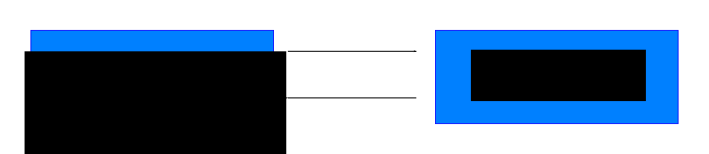
\includegraphics[width=0.8\textwidth]{arch-01.png}
  \end{center}

  \begin{itemize}
    \item<1-> Our system uses a basic client server model
    \item<2-> The client initiates all exchanges, the server replies
  \end{itemize}
\end{frame}

\begin{frame}[c]{High Level}
  \begin{center}
    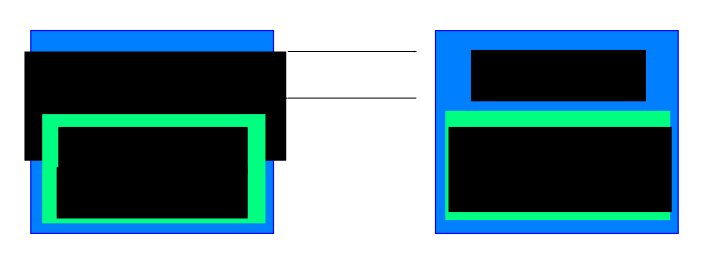
\includegraphics[width=0.8\textwidth]{arch-02.png}
  \end{center}

  \begin{itemize}
    \item<1-> The client side resides entirely in a single kernel module
    \item<2-> The server side is a standard userspace daemon
  \end{itemize}
\end{frame}

\begin{frame}[c]{Client Medium Level}
  \begin{center}
    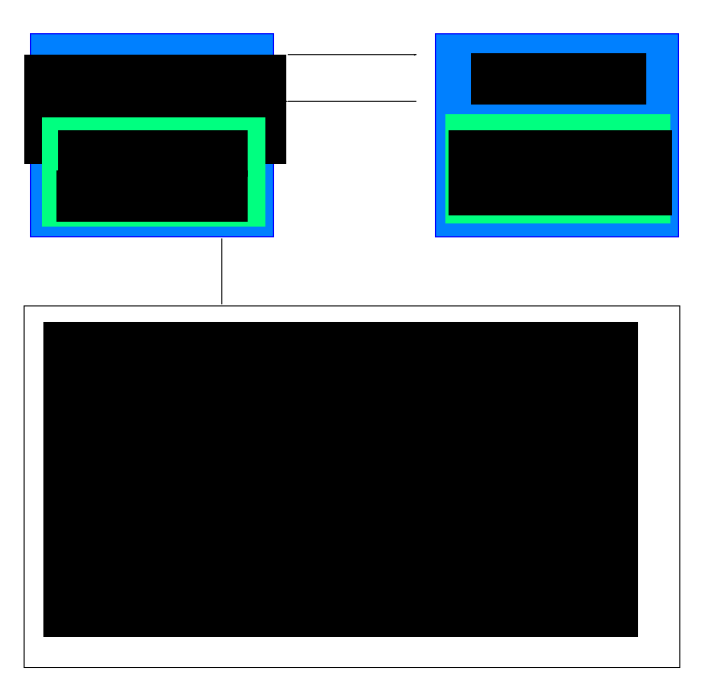
\includegraphics[width=0.4\textwidth]{arch-03.png}
  \end{center}

  \begin{itemize}
    \item<1-> By default, devices are exposed under \texttt{/dev/netchar}
    \item<2-> In the future, we should be able to choose any name
  \end{itemize}
\end{frame}

\begin{frame}[c]{Server Medium Level}
  \begin{center}
    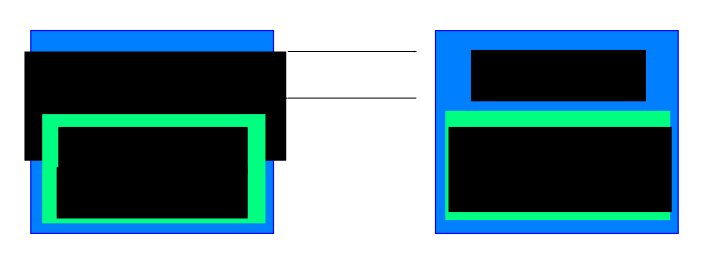
\includegraphics[width=0.8\textwidth]{arch-02.png}
  \end{center}
  \begin{itemize}
    \item<1-> Listen on a specified port
    \item<2-> Receive requests from client
    \begin{itemize}
      \item<2-> \texttt{open()},\texttt{close()},\texttt{read()},\texttt{write()},...
    \end{itemize}
    \item<3-> Can actually export \textit{any} file
    \item<4-> Crashes ungracefully when the client disconnects
  \end{itemize}
\end{frame}

\begin{frame}[c]{Protocol}
  \begin{center}
    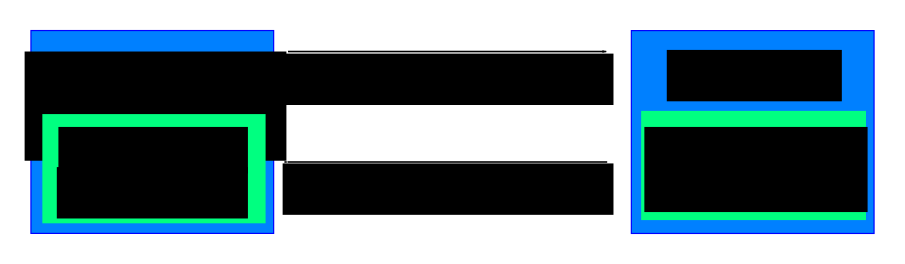
\includegraphics[width=0.8\textwidth]{proto.png}
  \end{center}

  \begin{itemize}
    \item<1-> Structures passed through \texttt{INET} socket
    \item<2-> Raw data immediately follows when necessary
    \begin{itemize}
      \item<2-> \texttt{read()}, \texttt{write()}, ...
    \end{itemize}
  \end{itemize}
\end{frame}


\section{Implementation}

\subsection{Protocol}

\begin{frame}[fragile]{Protocol}
  \begin{columns}
    \begin{column}{0.5\textwidth}
      \begin{lstlisting}[gobble=8]
        enum FOPS {
          FOP_OPEN, FOP_RELEASE,
          FOP_READ, FOP_WRITE,
          _FOP_ERROR
        };

        struct fop_request {

          enum FOPS call;

          union {
            struct {
              int     flags;
              mode_t  mode;
            };

            size_t  count;
          };
        };
      \end{lstlisting}
    \end{column}
    \begin{column}{0.5\textwidth}
      \begin{lstlisting}[gobble=8]
        struct fop_reply {

          enum FOPS call;

          union {
            int      open;
            int      close;
            ssize_t  read;
            ssize_t  write;
          };
        };
      \end{lstlisting}
    \end{column}
  \end{columns}
\end{frame}

\subsection{Client}

\begin{frame}[fragile]{Hello, World!}
  \begin{columns}
    \begin{column}{0.6\textwidth}
      \begin{lstlisting}[gobble=8]
        #include <linux/kernel.h>
        #include <linux/module.h>

        static int __init nc_init(void)
        {
          /* do stuff */
          return 0;
        }

        static int __exit nc_exit(void)
        {
          /* undo stuff */
        }

        MODULE_LICENSE("GPL");

        module_init(nc_init);
        module_exit(nc_exit);

      \end{lstlisting}
    \end{column}
    \begin{column}{0.4\textwidth}
      \begin{itemize}
        \item initial setup
        \item cleanup important!
      \end{itemize}
    \end{column}
  \end{columns}
\end{frame}

\begin{frame}[fragile]{Character Device Driver}
  \begin{lstlisting}[gobble=4]
    #include <linux/cdev.h>
    #include <linux/device.h>
    #include <linux/fs.h>

    static dev_t          nc_dev_t;
    static struct class*  nc_class;
    static struct cdev*   nc_cdev;
    static struct device* nc_device;

  \end{lstlisting}

  \begin{itemize}
    \item<1-> \texttt{dev\_t}: major/minor number
    \item<2-> \texttt{class}: subsystem
    \item<3-> \texttt{cdev}: handler for character devices
    \item<4-> \texttt{device}: userspace \texttt{/dev} node
    \item<5-> each has some form of registration mechanism
  \end{itemize}
\end{frame}

\begin{frame}[fragile]{Filesystem Handler}
  \begin{lstlisting}[gobble=4]
    #include <linux/fs.h>

    static int netchar_open(struct inode* inp, struct file* fp);
    static ssize_t netchar_read(struct file* fp, char* buffer,
                                size_t length, loff_t* offset);

    static struct file_operations nc_fops = {
      /* ... */
      .open  = nc_open,
      .read  = nc_read,
    }
  \end{lstlisting}

  \begin{itemize}
    \item<1-> required when registering character device
    \item<2-> buffer is a userspace pointer!
    \item<3-> event driven, blocking, asynchronous
  \end{itemize}
\end{frame}

\begin{frame}{Socket Client}
  \begin{itemize}
    \item<1-> socket type: \texttt{AF\_INET}, \texttt{SOCK\_STREAM}, \texttt{IPPROTO\_TCP}
    \begin{itemize}
      \item<2-> should be \texttt{AF\_NETLINK}
      \item<2-> do not want to lose messages
    \end{itemize}
    \item<3-> no familiar \texttt{read()}, \texttt{write()}
  \end{itemize}
\end{frame}

\subsection{Server}

\begin{frame}[fragile]{Server (\texttt{read()})}
  \begin{lstlisting}[gobble=4]
    struct fop_request req;
    struct fop_reply   rep;
    while (1) {
      err = read(sd, &req, sizeof(req));
      switch(req.call) {
      case FOP_READ:
        payload = realloc(payload, req.count);
        rep.read = read(fd, payload, req.count);
        if (rep.read < 0)
          rep.read = -errno;
        break;
      }
      err = write(sd, &rep, sizeof(rep));
      if (rep.call == FOP_READ && rep.read > 0)
        err = write(sd, payload, rep.read)
    }
  \end{lstlisting}
\end{frame}

\subsection{Misc}

\begin{frame}[t,fragile]{\texttt{udev}}
  \begin{lstlisting}[gobble=4,title=no way to set permissions within kernel,language=]
    ACTION=="add", SUBSYSTEM=="netchar", MODE="0666"
  \end{lstlisting}
  \begin{lstlisting}[gobble=4,title=cannot retroactively apply input attributes,language=]
    $ udevadm info -qall -n /dev/input/event8
    P: /devices/virtual/input/input8/event8
    N: input/event8
    E: DEVNAME=/dev/input/event8
    E: DEVPATH=/devices/virtual/input/input8/event8
    E: ID_INPUT=1
    E: ID_INPUT_KEY=1
    E: SUBSYSTEM=input
  \end{lstlisting}
\end{frame}

\begin{frame}[fragile]{\texttt{ncadmin}}
  \begin{lstlisting}[gobble=4,language=]
    usage: ncadmin command [args]

      The following commands are supported:

      add server port [name]
        server - an ip address
        port   - a port
        name   - optional name relative to /dev. if no name is
                 specified /dev/netchar/import# will be used

      rm name
        name   - the device relative to /dev to remove
  \end{lstlisting}
  \begin{itemize}
    \item<2-> does nothing!
    \item<3-> could use discovery service
    \item<4-> requires individual \texttt{cdev}s
    \item<5-> name is optional
  \end{itemize}
\end{frame}

% Matt - End

% Andy Sections

\section{Results and Evaluation}
%---Full State Slide---%

\begin{frame}[c]{Full System}
  \begin{center}
    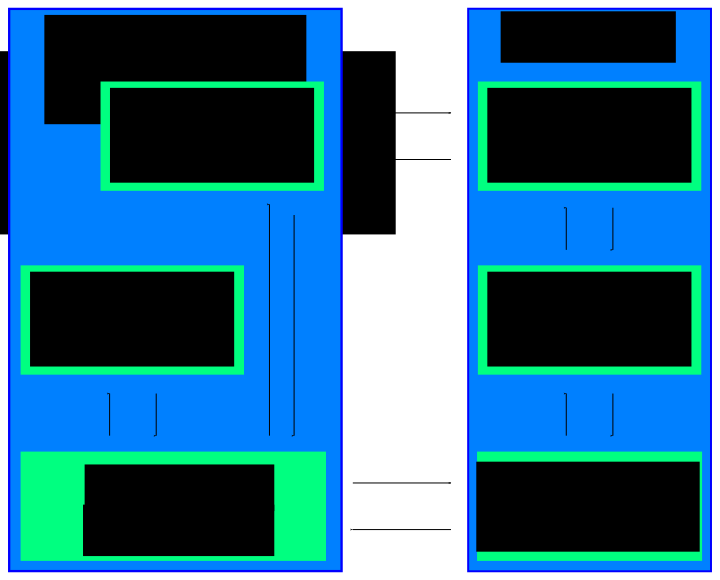
\includegraphics[height=0.75\paperheight,keepaspectratio]{system-full.png}
  \end{center}
\end{frame}

%---Current State Image Slide---%
\begin{frame}[c]{Current State}
  \begin{center}
    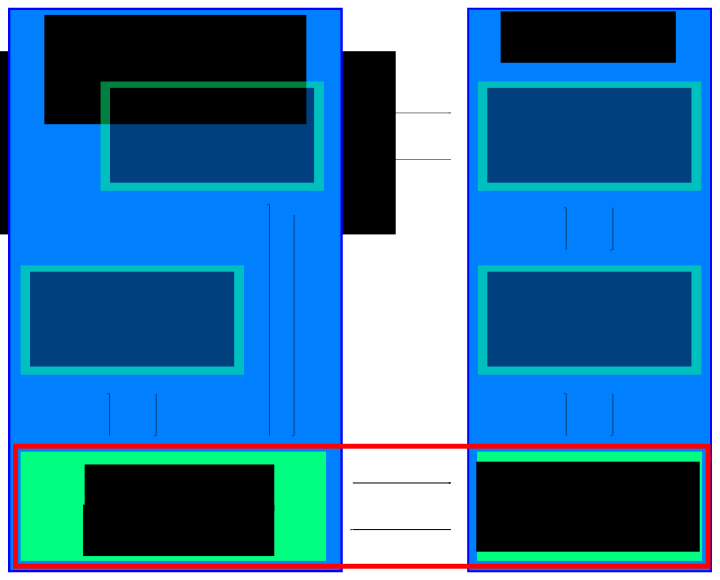
\includegraphics[height=0.75\paperheight,keepaspectratio]{system-working.png}
  \end{center}
\end{frame}

%---Current State Slide---%
\begin{frame}{\bf Current State}

  \begin{itemize}
  \item<1-> Supports exporting a single character device from the server
  \item<2-> Supports importing a single character device on the client
  \item<3-> Supports open, close, read, and write calls
  \item<4-> Supports basic Linux udev operation for automatic node
    creation on client
  \item<5-> Tested with various ``real'' and device files
  \end{itemize}

\end{frame}

%---ToDo Slide---%
\begin{frame}{\bf ToDo}

\begin{itemize}
\item<1-> Multi-device, multi-server client-side import support
\item<2-> Multi-device server-side export support
\item<3-> Support for exclusive use and protection of exported devices
\item<4-> Support for ioctl calls
\item<5-> Support for providing and obtaining metadata for exported
  devices
\item<6-> Support for ``advertisement'' of available exported devices
\item<7-> Support for integrating imported devices into other kernel
  subsystems (human interface subsystem, audio subsystem, etc)
\item<8-> Addition of ``NCD-admin'' utilities for managing and administering
  NCD system
\item<9-> Addition of graceful connect and disconnect handling in real-time
\end{itemize}

\end{frame}

%---Advantages Slide---%
\begin{frame}{\bf Advantages}

What are the benefits of using Networked Character Device?

\begin{itemize}
\item<1-> Divorces peripherals from the computers to which they are
  attached
\item<2-> Allows simple creation of a ``Device Server''
\item<3-> Extends the ``Everything Is A File'' -nix Philosophy
\item<4-> Allows more efficient use of devices
\item<5-> Allows devices to be networked in a generalized, uniform manner
\end{itemize}

\end{frame}

%---Challenges Slide---%
\begin{frame}{\bf Challenges}

But there are difficulties making it work on a production scale...

\begin{itemize}
\item<1-> Does not work well when Character Device is not the exclusive
  device interface
  \begin{itemize}
  \item Many modern day devices interface directly with other
    in-kernel function, interfaces, and APIs
  \item procfs and sysfs provide additional device interface points
  \item Socket interfaces (netlink, etc) provide alternative to file
    system interfaces
  \end{itemize}
\item<2-> Requires exported devices to be ``de-integrated'' from host system
\item<3-> Requires QOS guarantees and high guilty network connection
\end{itemize}

\end{frame}

%---Potential Uses Slide---%
\begin{frame}{\bf Potential Uses}

What can we use NCDs for?

\begin{itemize}
\item<1-> Quick, cheap, and simple ad-hoc network KVM systems
\item<2-> Remote, networked web-cams, scanners, printers, etc
\item<3-> Basis of ``protocol''-over-Ethernet systems (USB-over-Ethernet,
  SATA-over-Ethernet, Etc)
\item<4-> Basis of redundant, ``cloud-like'' device pools
\item<5-> Basis of peripheral cluster systems (GPU Clusters, RNG Clusters,
  Etc)
\end{itemize}

\end{frame}

%---KVM Slide---%
\begin{frame}{\bf KVM}

Building a networked KVM system with NCDs:

  \begin{center}
    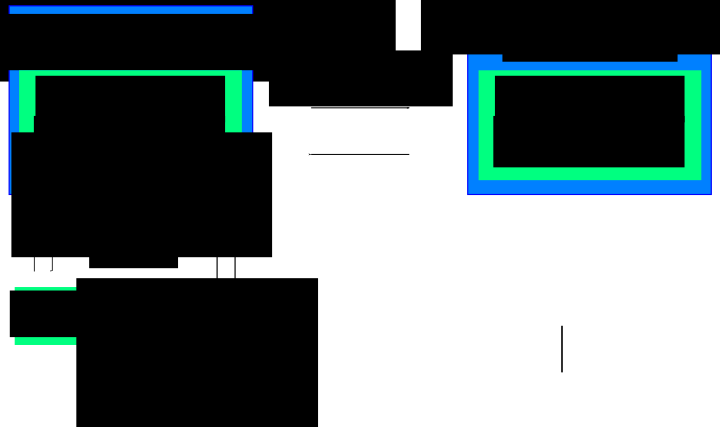
\includegraphics[height=0.6\paperheight,keepaspectratio]{kvm.png}
  \end{center}

\end{frame}

%---Device Pool Slide---%
\begin{frame}{\bf Random Number Generator Pool}

Building a distributed RNG system with NCDs:

  \begin{center}
    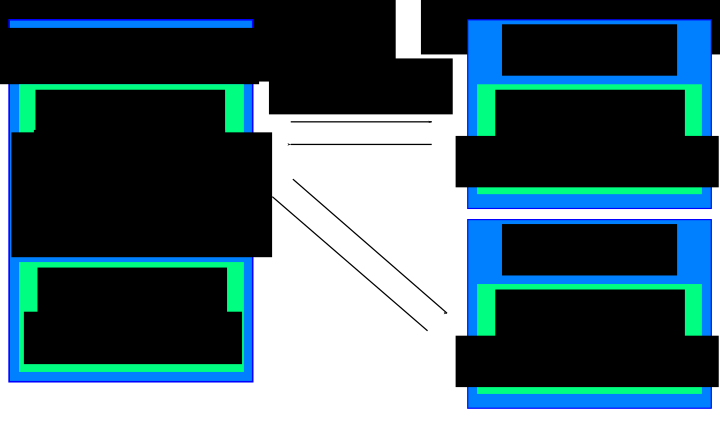
\includegraphics[height=0.6\paperheight,keepaspectratio]{rng.png}
  \end{center}

\end{frame}

\section{Future Work}
%---Potential Uses Slide---%
\begin{frame}{\bf Future Work}

\begin{itemize}
\item<1-> Add multi-device, multi-server support
\item<2-> Add kernel sub-system handler layer (HID, etc)
\item<3-> Add device protection and removal capabilities to server system
\item<4-> Add advertisement protocol
\item<5-> Consider removing networking code from client kernel module
\end{itemize}

\end{frame}

\section{Conclusion}

%---Conclusion Slide---%
\begin{frame}{\bf Conclusion}

Network Character Devices provide:

\begin{itemize}
\item<1-> A simple means to add network functionality to devices using
  well understood file semantics and interfaces.
\item<2-> The groundwork for cloud-like device pools and arrays
\item<3-> The means to efficiently export devices from where they are not
  need and import them where they can be used.
\end{itemize}

But to make them widely applicable:

\begin{itemize}
\item<4-> Device drivers must move back toward the sole use of the
  device file based APIs
\item<5-> Advertisement and management tools must be added
\item<6-> The OS must not assume that it has exclusive access to any
  device connected to the physical hardware on which it is running.
\end{itemize}

\end{frame}

\section{Bibliography}

%---Bibliography---%
\begin{frame}[t,allowframebreaks]{\bf Bibliography}
\nocite{*}
\bibliography{refs}
\end{frame}

\end{document}

% vim: set sw=2 ts=2 sts=2 et spell : %
